Während der letzten Jahrzehnte hat sich die Rolle der IT innerhalb eines Unternehmens gravierend verändert. Diese bestand darin, Geschäftsprozesse zu unterstützen und skalierbare IT-Dienste bereitszustellen \cite{haffke_transformative_2017}, die auf betriebliche Kosteneffizienz ausgelegt waren und wodurch die gesamte Unternehmenslandschaft statisch aufgebaut war. \cite[S. 16]{ravichandran_devops_2016} Aufgrund der Globalisierung und des technologischen Fortschrittes sind heutige Geschäftsmodelle immer komplexer und schnelllebiger, wodurch die größte Herausforderung für Unternehmen darin besteht, kontinuierlich innovativ und schlank zu bleiben. \cite{haffke_transformative_2017} Die daraus resultierende Verschiebung zeigt, dass IT eine zunehmend zentrale Rolle für Unternehmen einnimmt und als ein Enabler agiert um weiterhin wettbewerbsfähig zu bleiben. \cite{haffke_transformative_2017} Wesentlicher Kernaspekt der IT ist die Softwareentwickung.\\\\ In den Anfangsjahren der Softwareentwicklung lag der Schwerpunkt auf den Bereich der Anforderungen, wodurch die Modelle starken Kontrollen und strukurierten Vorgehen unterlagen. \cite{kneuper_sixty_2017} Als eines der bekanntesten, traditionellen Softwareentwicklungsmodellen gilt das Wasserfallmodell, welches sich durch eine prozessorientierte Entwicklung kennzeichnet. \cite{bakaji_waterfall_2012} Dabei werden bereits vor Projektbeginn alle Anforderungen gesammelt und klassifiziert, um die Sofware dahingehend zu entwickeln und zu testen. Infolgedessen werden die Anforderungen zwar klar und in einem festgelegten Zeitraum festgelegt \cite{bakaji_waterfall_2012}, können sich allerdings im Laufe des Projeks ändern, wenn neue Lösungen in Betracht gezogen werden müssen. Infolgedessen ist für die gesamte Softwareentwicklung hinweg viel mehr Flexibilität erforderlich, insbesondere bei der Nachfrage der Kunden oder der Stakeholder nach immer besseren und schnelleren Softwareprodukten. \cite[S. 17]{ravichandran_devops_2016} \\\\ Die daraus entstehende Veränderung verursachte eine Anpassung der gängigen Praktiken und Vorgehensweisen innerhalb des IT-Bereichs. Anfang des 21. Jahrhunderts kamen agile Methode auf, die in der Softwareentwicklung etabliert worden sind. Gründe waren der wachsende Time-to-Market und der zunehmende Wettbewerb, teilweise bedingt durch das Aufkommen des World Wide Web und die daraus resultierende Notwendigkeit, sich besser an unklare oder ändernde Anforderungen anzupassen. \cite{haffke_transformative_2017} Bei der agilen Softwareentwicklung handelt es sich einerseits um eine iterative Arbeitsweise, die sich aus unterschiedlichen Methoden und Techniken zusammensetzt und anderseits um ein Mindset, welches durch die unterschiedlichen Tools und Techniken unterstützt wird. Kernaspekte sind dabei die Aufnahme von kontinuierlichen Anpassungen anhand von neuen oder veränderten Anforderungen innerhalb des Gesamtprozesses, Begrenzung der Dokumentation auf das Wesentliche und die Arbeitsweise mit kleinen und regelmäßigen Iterationen in überschaubaren Inkrementen. \cite{cohen_introduction_2004}, \cite{bakaji_waterfall_2012}, \cite[S. 18]{ravichandran_devops_2016} Durch eine iterative Problemlösung und häufiges Feedback, können komplexe Geschäftsprozesse gelöst und damit die fortlaufende Zufriedenheit der Kunden sichergestellt werden. Vorteilhaft ist, dass sich Unternehmen schnell an neue Informationen anpassen, Fehler früher gefunden werden, sofortige Verbesserungen der Software durchgeführt wird, Lernfortschritt erhöht und eine schnelle Entwicklung und Auslieferung möglich ist. \cite[S. 18]{ravichandran_devops_2016} Insgesamt war die wachsende Bedeutung der Technologie im Zeitalter der Digitalisierung, die sich mittelbar auf das Geschäftsleben oder insbesondere auf den Bereich der Softwareentwickung ausgewirkt hat, letztlich der Grund für die Einführung von DevOps. \cite{haffke_transformative_2017} Obwohl der Begriff 'DevOps' das erste Mal von Patrick Debois geprägt worden ist, als er im Jahr 2009 die erste DevOpsDays-Veranstaltung in Gent/Belgien organisierte, liegen die Ursprünge dieses Konzepts weit früher. \cite[S.3]{kim_devops-handbuch_2017} Die Wurzeln können zunächst im Bereich der Lean-Bewegung angesehen werden, welches darauf basiert, dass das hergestellte Produkt kontinuierlich verbessert, Verschwendung vermieden, auf schnelles Feedback und kürzeres Time-to-Market setzt. \cite[S.2]{kim_devops-handbuch_2017} \cite{nelson_devops_2016} \cite[S. 11]{ravichandran_devops_2016} Letztlich wurde dieser Grundgedanke am Anfang des 21. Jahrhunderts aufgegriffen und mit dem Konzept des agilen Manifestes \cite{beck_manifesto_2001} erweitert.\\\\ Zu dieser Zeit war ein generelles Problem, dass Entwickler Softwareänderungen und Updates schnell liefern konnten, aber der Betrieb, der die Verfügbarkeit von Anwendungen gewährleistet, diese Funktionen nur langsam bereitgestellen konnte, da dieser starre Änderungsmanagementprozesse hatte. Dieses Problem wird oftmals als \textit{Wall of Conflict} bezeichnet und beschreibt Probleme im Arbeitsfluss durch fehlende Informationen, wie Abbildung 1 schematisch zeigt. \cite{kawaguchi_wall_2020}, \cite[S. 26]{huttermann_devops_2012} 

\begin{figure}[h]
    \centering
    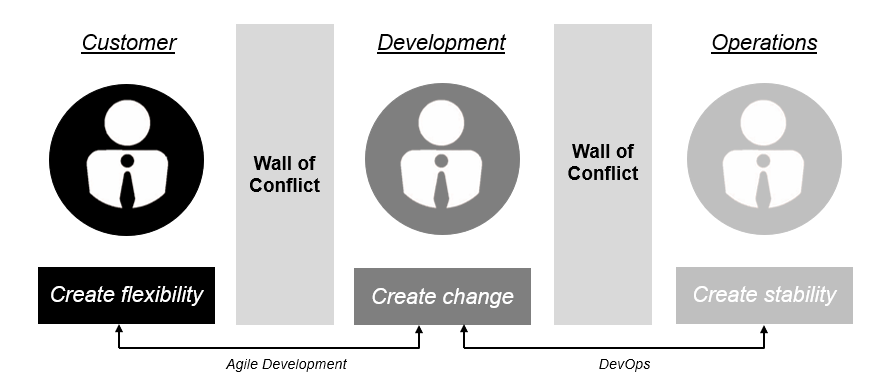
\includegraphics[scale=0.6]{Bilder/Wall of Conflict.png}
    \caption{Wall of Conflict, angelehnt an \cite{hering_devops_2018}}
\end{figure}

Gründe dafür waren, dass sowohl Entwickler- als auch Betriebsteam unterschiedliche Ziele, Denkweisen und Prozessen verfolgt haben. \cite{wettinger_streamlining_2016} Der daraus resultierende Engpass führte zu einem erheblichen Mehraufwand insbesondere im Bereich des Ops-Teams und zu verspäteten Auslieferungen von Softwareprojekten. Mittels des DevOps-Ansatzes sollen die Silos zwischen der Entwicklung des Betriebs aufgebrochen werden, indem kleine und funktionsübergreifende Teams gebildet werden, die die DevOps-Praktiken und Prinzipien verfolgen. \cite{ebert_devops_2016}, \cite{wiedemann_research_2019} In diesem Rahmen werden automatisierte Pipelines aufgebaut, um manuelle Arbeiten zu reduzieren und eine kontinuierliche Bereitsstellung sicherzustellen. \cite[S.3,5]{verona_practical_2016} Demnach sollte einerseits eine dauerhafte Interaktion mit dem Kunden stattfinden und andererseits keine Messung von großen Meilensteinen mehr erfolgen. \cite[S.5]{sharma_devops_2017}\\\\ Aus diesem Grundgedanken heraus, handelte es sich bei dem DevOps-Ansatzes zunächst um eine kulturelle Bewegung, die die Unterschiede zwischen Dev und Ops verändern sollte und die Bereitstellung mittels Automatisierung, schneller, effizienter und kontinuierlicher zu gestalten. \cite[S.5]{sharma_devops_2017} Letztlich kann DevOps nicht als ein vollständig neuer Ansatz, sondern vielmehr als eine Weiterentwicklung bereits bekannter Konzepte angesehen werden. \cite[S. 23]{alt_innovationsorientiertes_2017}

